\documentclass[polish,twoside]{article}

% pakiet MwE
\usepackage{ze}

% tytul referatu
\title{Uwagi odnośnie redakcji artykułów do Zeszytów Energetycznych}
\shorttitle{Uwagi redakcyjne...}
% tytul referatu w jez. angielskim
\titleEng{Tytuł referatu w języku angielskim}
% Autorzy
\author{Jerzy Kulej\affmark[1], Dominik Bajoński\affmark[2]}
% Autorzy nagłówek
\authorheader{Jerzy Kulej}
% Afiliacje autorów
\affiliations{
    \affaddr[1]{Politechnika Kaliska, Katedra Procesów Cieplno-Przepływowych}
    \affaddr[2]{Politechnika Wrocławska, Katedra Turbin i Modelowania Procesów Cieplno-Przepływowych}
}
% Kontaktowy adres mailowy
\contactaddress{ze@pwr.edu.pl}

\begin{document}

\maketitle

\begin{ZEabstract}
Podano, uwagi odnośnie  długości i redakcji tekstu.
\end{ZEabstract}

\begin{keywords}
\LaTeX, tylda, rysunki .
\end{keywords}

\normalsize

\section{Wprowadzenie}

Prosimy o przygotowanie artykułu według szablonu \textbf{szablonZeszyty} i stylu ze.sty.
Plik szblonu \textbf{ ze.sty} musi znajdować się w katalogu, w którym piszemy i  kompilujemy nasz artykuł. Tekst kompilujemy używając\textbf{ PdfLatex}. Powstaje od razu wersja .pdf. Wersję źródłową \emph{nazwisko}.tex i wersję \emph{nazwisko}.pdf wraz z rysunkami należy przesłać na adres \textbf{ze@pwr.edu.pl}.

Zbiory z rysunkami nazywamy rysunek1, rysunek2, .. itd. w kolejności takiej jak się pojawiają w tekście artykułu. Koniecznie poddać szczegółowemu sprawdzeniu artykuł w formacie .pdf. Rysunki wstawiamy w formacje *.jpg lub *.png.  W preambule należy wpisać tytuł swojego referatu i inne swoje dane.
Niepotrzebne, struktury "zawieszamy" stawiając na początku linii znak \%. 

Pierwszy raz kompilujemy dwukrotnie aby zostały wypełnione odwołania do literatury. Pozycje literaturowe  podawać zgodnie ze wzorcem. Starać się zachować kolejność alfabetyczną. Cytujemy używając np. \textbf{$\backslash$cite}\{Aref1\}  co utworzy \cite{Aref1}. Literaturę zamieszczamy według wzoru podanego na końcu niniejszego wprowadzenia . Na stronie zeszytów \textbf{www.ze.pwr.edu.pl} zostanie zamieszczony  prosty podręcznik do \LaTeX'a. Wszelkie inne informacje również będą zamieszczane na tej stronie internetowej. Można zwrócić się o pomoc do Panów dr hab. Sławomira Pietrowicza   lub do mnie (Henryk Kudela). Wielu kolegów posługuje się już świetnie \LaTeX'em, więc do nich również można się zwrócić o pomoc. Istnieje wiele tutoriali, podręczników. Polecanie godnym jest łatwo dostępna  publikacja Tobiasa Oetikera i innych: \textbf{Nie~za~krótkie wprowadzenie do systemu \LaTeX 2}.

\section{Szczegółowe uwagi odnośnie redakcji artykułów}
Wcześniejsza praca nad redakcją Zeszytów pozwala sformułować kilka dodatkowych uwag, których uwzględnienie byłoby niezwykle pożyteczne:
\begin{enumerate}
    \item Należy zwrócić uwagę na czytelność zamieszczanych w tekście rysunków. Dla zachowania czytelności czcionka na rysunkach powinna być tej wielkości co podpis pod rysunkiem. Unikać zdjęć stanowisk doświadczalnych, zdjęć dokumentujących odczyty z przyrządów,
    \item Zwrócić uwagę, aby koniec linii nie kończył się pojedynczą literą , np. w, z, i itp. (tzw. zawieszki). Odstępy, na których nie wolno złamać wiersza, zaznacza się w pliku źródłowym przez umieszczenie znaku tyldy \~{}  zamiast odstępu np.~ w\~{}~końcu.
    \item  Pojedyncze zadanie zamykające akapit nie może przenosić się na nową stronę. Należy tak formatować tekst, dobierając wielkość rysunków i ich położenie, aby wymusić zachowanie ciągłość myśli wyrażonej w tekście. Do dyspozycji jest jeszcze instrukcja \textbf{newline}. Nową myśl (akapit) powinniśmy zaczynać wcięciem. Jeżeli Latex tego nie zrobił automatycznie to można to wymusić instrukcją  \indent.
    \item Wzory  chemiczne  jak również wymiary jednostek fizycznych piszemy prosto. Aby skorzystać z możliwości trybu matematycznego pisania indeksów można użyć  instrukcji  \text{$\backslash$operatorname}. Miedzy liczbą a jednostką fizyczną pozostawimy spację np. 1 m$^2$. Natomiast nie ma spacji przy wielkości wyrażającej  temperaturę  w stopniach Celsjusza, no 1$^o$C.
    \item Jeżeli we worze matematycznym został użyty symbol i jest on używany w tekście to musi być napisany italikiem (pochyło),
    \item Artykuł powinien zawierać parzystą liczbę stron, nie mniej niż 8. 
\end{enumerate}

\section{Przykłady wzorów matematycznych}
Przykład fragment tekstu z \textbf{równaniami} zamieszczono poniżej.
Równania ruchu lepkiego i nieściśliwego płynu mają postać (równanie \ref{eom} oraz \ref{incmp} - odniesienie do równania zapisujemy jako np. $\backslash$ref\{eom\}, natomiast równanie ma dodany $\backslash$label\{eom\}, który tworzy podstawę odniesienia):
\begin{equation}\label{eom}
\frac{\partial{\mathbf{u}}}{\partial t}+(\mathbf{u} \cdot \nabla)\mathbf{u}=-\frac{1}{\rho}\nabla p+\nu \Delta \mathbf{u},
\end{equation}
\begin{equation}\label{incmp}
\nabla \cdot \mathbf{u}=0,
\end{equation}
gdzie $\mathbf{u}=(u,v,w)$ jest wektorem prędkości, $\rho$ -- gęstością płynu, $p$ -- ciśnieniem a $\nu$ -- kinematycznym współczynnikiem lepkości.

\section{Przykład zamieszczania wykresów, obrazków.}

W dalszej części przedstawiono przykłady zamieszczania \textbf{wykresów, obrazków oraz tabel.}
Pojedynczy wykres lub zdjęcie (Rys. \ref{obraz1} - odniesienie do obrazu tworzymy analogicznie do przykładu z równaniem):
\begin{figure}[h!]
\centering
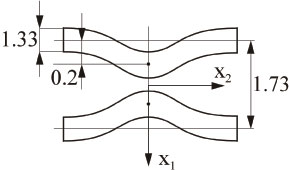
\includegraphics[width=0.45\linewidth]{figure1.jpg}
\caption{Jeden obrazek z podpisem}\label{obraz1}
\end{figure}

Dwa wykresy lub zdjęcia obok siebie z dwoma niezależnymi popisami (Rys \ref{obraz2} oraz Rys. \ref{obraz3}):

\begin{figure}[htb]
\centering
\begin{minipage}[t]{0.42\linewidth}
\centering
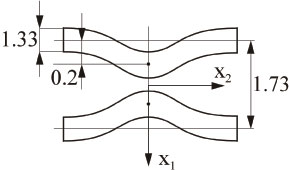
\includegraphics[width=0.65\linewidth]{figure1.jpg}
\caption{Dwa obrazki obok siebie z dwoma podpisami (lewy)}\label{obraz2}
\end{minipage}
\quad
\begin{minipage}[t]{0.42\linewidth}
\centering
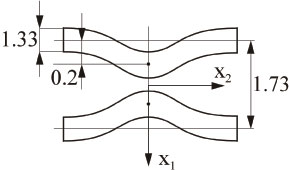
\includegraphics[width=0.65\linewidth]{figure1.jpg}
\caption{Dwa obrazki obok siebie z dwoma podpisami (prawy)}\label{obraz3}
\end{minipage}
\end{figure}

Przykład tworzenia tabeli (Tab. \ref{tab1} oraz Tab. \ref{tab:cryocoolers}).\\
\begin{table} [!ht]
\caption{Przyspieszenie osiągane dla metody Jacobiego.}\label{tab1}
\centerline{
\begin{tabular}{|c|c|c|c|c|}
\hline
Liczba węzłów & tsl  &  tx &  nc & frm nc\\
\hline
32x32x32 & 4.05 & 6.61 & 6.94 & 12.32\\
64x64x64 & 17.71 & 26.32 & 31.26 & 52.82\\
128x128x128 & 24.78 & 29.95 & 43.67 & 58.89\\
\hline
\end{tabular}}
\end{table}

Dodatkowy przykład tworzenia tabeli.\\
\begin{table}[h]
    \centering
    \caption{Cryogenic coolers}
    \label{tab:cryocoolers}
    \begin{tabular}{@{}lll@{}}
    \toprule
    \begin{tabular}[c]{@{}c@{}}Cryooler\end{tabular} &
      \begin{tabular}[c]{@{}c@{}}Capacity range\end{tabular} &
      \multicolumn{1}{c}{ } \\ \midrule
    \begin{tabular}[c]{@{}c@{}}Turbo-Brayton\end{tabular}    & 18 - 250 kW at 120 K  \\
    \begin{tabular}[c]{@{}c@{}}Stirling\end{tabular}         & 2 - 8 kW at 120 K     \\
    \begin{tabular}[c]{@{}c@{}}Gifford-McMahon\end{tabular}  & 14 - 600 W at 80 K     \\
    \begin{tabular}[c]{@{}c@{}}Single-stage Pulse Tube\end{tabular}  & 12 - 90 W at 80 K  \\
    \begin{tabular}[c]{@{}c@{}}Miniature Pulse Tube\end{tabular}       & 3 - 10 W at 80 K    \\
    \begin{tabular}[c]{@{}c@{}}Joule-Thomson\end{tabular}       & 100 W at 120 K   \\ \bottomrule
    \end{tabular}
\end{table}


\section{Podsumowanie}

W pracy przedstawiona została implementacja metody cząstek wirowych typu „wir w komórce” wykorzystująca metodę dekompozycji lepkościowej.

\begin{thebibliography}{10}
{\small
\bibitem{Aref1} Aref H.  \textit{Motion of three vortices}, Phys. Fluids \textbf{22} (3), 393-400, 1997
\bibitem{Holden_etal_2007} Holden H., Karlsen K.H., Lie K.-A., Risebro W.H. \textit{Splitting Methods for Partial Differential Equations with Rough Solutions}, Society for Industrial and Applied Mathematics,  2007
\bibitem{LeVeque_2010} LeVeque R.J. \textit{Finite Difference Methods for Ordinary and Partial Differential Equations}, European Mathematical Society, 2010
\bibitem{Kudela_Kosior_2013} Kudela H., Kosior A. \textit{Parallel reconnection of vortex tube reconnection using a graphics card and the 3D Vortex-in-Cell method}, Procedia IUTAM, \textbf{7}, 59-66, 2013

}
\end{thebibliography}
\end{document}
